\documentclass{beamer}
 
\usepackage[utf8]{inputenc}

\usetheme{Madrid}
 
%Information to be included in the title page:
\title[ZPP] %optional
{Framework oparty o wzorzec mikrousług na przykładzie portalu dla ZUS}
 
\subtitle{}
 
\author[Jaroń, Socha, Zalas] % (optional, for multiple authors)
{Michał Jaroń \and Jarosław Socha \and Piotr Zalas}
 
\institute[MIMUW] % (optional)
{
}
 
\date[9 czerwca 2017] % (optional)
{}
 
\begin{document}

\frame{\titlepage}
 
\begin{frame}
\frametitle{TODO}
This is a text in first frame. This is a text in first frame. This is a text in first frame.
\end{frame}

\begin{frame}
\frametitle{Architektura naszej aplikacji}
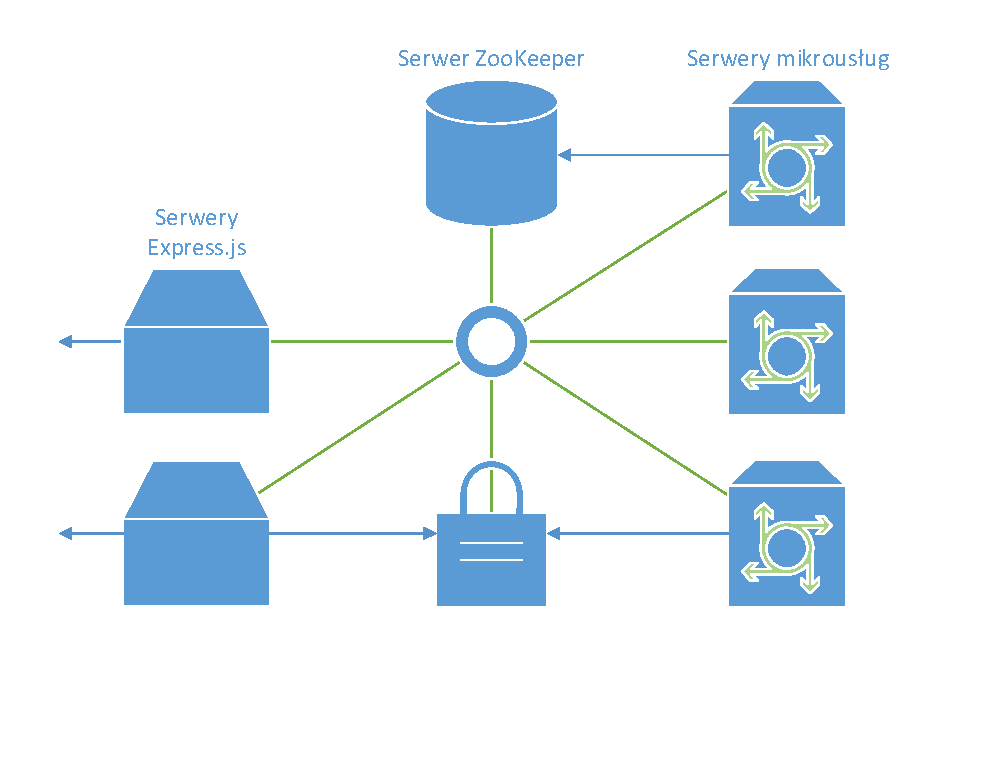
\includegraphics[width=\textwidth]{calosc.pdf}
\end{frame}

\begin{frame}
\frametitle{Architektura naszej aplikacji - Frontend}
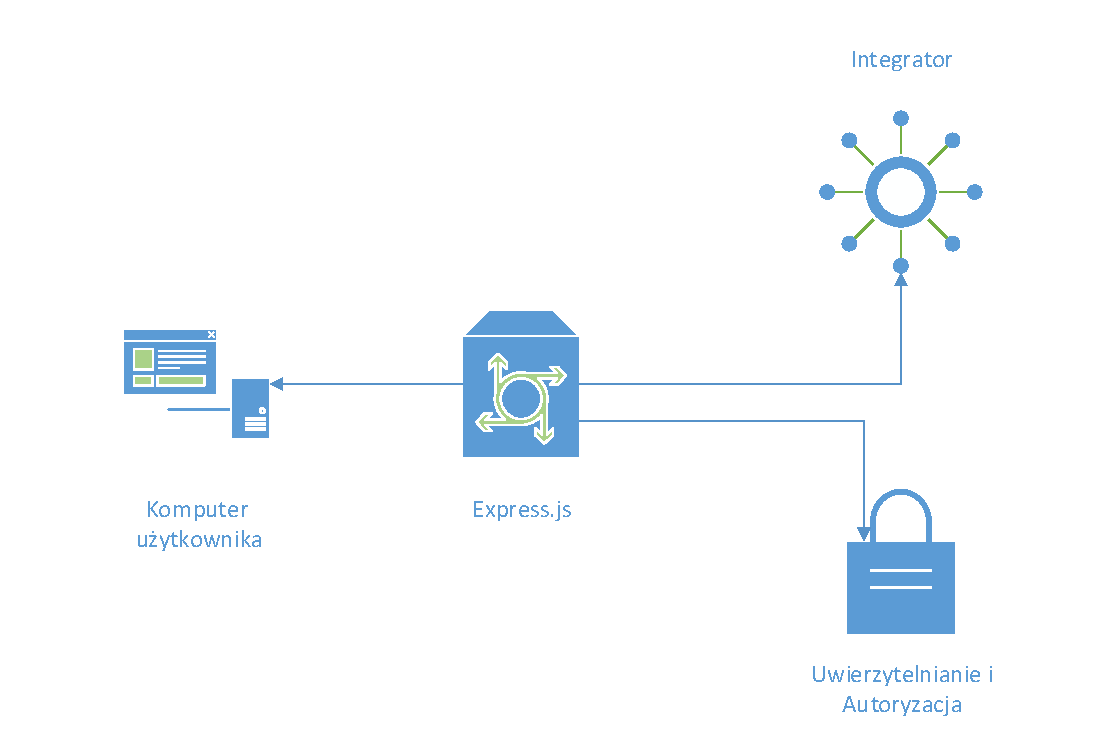
\includegraphics[width=\textwidth]{Frontend.pdf}
\end{frame}

\begin{frame}
\frametitle{Architektura naszej aplikacji - Backend}
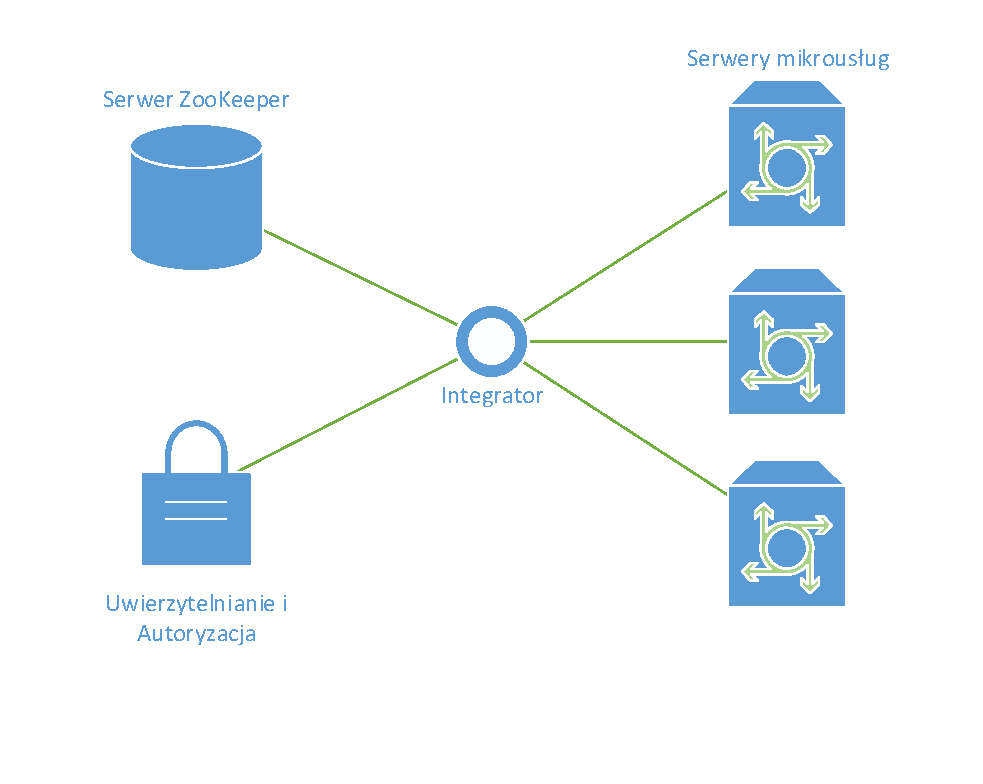
\includegraphics[width=\textwidth]{backend.pdf}
\end{frame}

\begin{frame}
\frametitle{Sample frame title}
 
In this slide, some important text will be
\alert{highlighted} beause it's important.
Please, don't abuse it.
 
\begin{block}{Remark}
Sample text
\end{block}
 
\begin{alertblock}{Important theorem}
$\left\{{n}\atop{k}\right\} = % Liczba stirlinga = 
\sum_{1\le i_1\le i_2 \le \ldots \le i_{n-k}\le k} % Suma po ... z
i_1\cdot i_2\dots i_{n-k}$ % ... składników
\end{alertblock}
 
\begin{examples}
Sample text in green box. "Examples" is fixed as block title.
\end{examples}
\end{frame}

\begin{frame}[fragile]
\frametitle{Sample frame title}
 
Very important algorithm
Done

\end{frame}

\begin{frame}
\begin{itemize}
	\item This one is always shown
	\item<1-> The first time (i.e. as soon as the slide loads)
	\item<2-> The second time
	\item<1-> Also the first time
	\item<1-1> {This one is shown at the first time, but it will hide soon (on the next event after the slide loads).}
\end{itemize}
\end{frame}

\begin{frame}[fragile]{Example of columns 2}
	\begin{columns}[T] % contents are top vertically aligned
		\begin{column}[T]{5cm} % each column can also be its own environment
			Contents of first column \\ split into two lines
		\end{column}
		\begin{column}[T]{5cm} % alternative top-align that's better for graphics
aaa
		\end{column}
	\end{columns}
\end{frame}

\end{document}
